\chapter{Research questions and Methodology}
% Methodology:
% - How do we answer RQs: simulation, controlled experiments, etc.

\section{Formalization of recurrent change detection}
% Formalization of recurrent change detection
% Nikolai: likely current 2.9 (Recurrency) and some 2.10 (Pccf) goes here
\section{Recurrency}

Adaptive learning in concept drift.
Predictability of events in the data stream.
~\cite{feller2008introduction}
Sums of independent random variables.
Recurrency is a form of predictability.

\subsection{Relevant material from Feller textbook}

The basic theory is as follows~\cite{feller2008introduction}.
In a sequence of Bernoulli trials the waiting time up to the first event gas a geometric distribution.
After the first event the process starts anew, and the number of trials between $n$ and $n+1$ th events has the same geometric distribution.
\begin{definition}
	Let $a_1, a_2, \dots, $ be a sequence of real numbers. If 
	\begin{equation}
		A(s) = a_0 + a_1 s + a_2 s^2 + \dots 
	\end{equation}
    converges in some interval $-s_0 < s < s_0 $ , then $A(s)$ is called the generarating function of the sequence $\{a_j\}$. 
\end{definition}

From\cite{wasserman2013all}
\begin{definition}
	The moment generating function MGF, or Laplace transform, of $X$ is defined by
	\begin{equation}
		\psi_X = \mathbb{E}(e^{tX}) = \int e^{tX} dF(x) 
	\end{equation}
where $t$ varies over the real numbers.
\end{definition}

\subsection{Inter-arrival times modeling}

Basic theory.
\begin{definition}
	A function $\mathbb{P}$ that assigns a real number $\mathbb{P}(A)$ to each event $A$ is a probability distribution if \\
	Axiom 1: $\mathbb{P}(A) \geq 0$ for every $A$\\
	Axiom 2: $\mathbb{P}(\Omega) = 1$\\
	Axiom 3: If $A_1, A_2, \dots $ are disjoint then 
	\begin{equation}
		\mathbb{P} \Big( \bigcup\limits_{i=1}^{\infty} A_i  \Big) = \sum_{i=1}^{\infty} \mathbb{P}(A_i)
	\end{equation}
\end{definition}
Commonly used probability distributions for modelling inter-arrival times.


\section{Pccf}~\label{sec:pccf}

If change points are expected to reoccur in the input signal, then this prior information can be used to approximate prediction time intervals, or regions of interest (ROI), where changes are most likely to appear in the future.
Once calculated, and if predictions are correct, then this information can further be used to reduce the false alarm rate of the change detection process, and potentially to reduce detection delays too.
FA rate can be decreased just by disregarding detections outside prediction intervals, and the detection delay can be decreased by increasing sensitivity of the detector within prediction intervals.
But, as mentioned, if sensitivity is increased, then probability of FA events will also increase.
Possibility of decreasing detection delays in the presence of prediction interval is a subject of Experiments section.
We describe next how to calculate prediction intervals for reoccurring change points.

To calculate ROIs for recurrent change points we use a prediction confidence change function (Pccf) proposed in our previous work~\cite{MaslovSDM2016}, where it was calculated using convolutions.
Below we calculate Pccf for several commonly used distributions of inter-arrival times values using moment generating functions, what is a more concise way than when using convolutions.
Let's start with definitions.
\begin{definition}
	Change points $t_i^{\text{c}}$ are recurrent if their inter-arrival times $t_{i}^{c} - t_{i-1}^{c}$
	% \begin{equation}\label{eq:recurrence_relation}
	%     \Delta_i = t_{i}^{c} - t_{i-1}^{c}
	% \end{equation}
	are i.i.d.\ from the same probability distribution.
	E.g., $t_{i}^{c} - t_{i-1}^{c} \sim \mathbb{N}(\mu, \sigma)$ if $\sigma$ is small.
\end{definition}
%The recurrence relation for recurrent changes is \begin{equation} x_{n+1} = x_n + \delta_n \end{equation}
Pccf function value at time moment $t_i$ is a probability estimator of recurrent change point to occur at this time moment.
%Recurrent changepoints form a sequence determined by recurrence relation given by Equation~\ref{eq:recurrence_relation}.
% $t_{i}^{\text{CHP}} = t_{i-1}^{\text{CHP}} + \Delta_i$.
Pccf can be represented as a matrix~\ref{eq:pccf_matrix} in which elements at row $k$ and column $i$ are probability estimates for change point $t_k^{\text{c}}$ to appear at time moment $t_i$.
\begin{equation}~\label{eq:pccf_matrix}
	\text{PCCF}_{k,i} \equiv P(t_{k}^{\text{c}} = t_i) % \: \forall \:  k, i \in [1,\dots,N
\end{equation}
When calculating ROIs we are interested in total probability of any changepoint occurring at every time moment within prediction horizon.
Since events $t_k^{\text{c}} = t_i$ are disjoint we need to sum up rows of the matrix $\text{PCCF}_{k,i}$
\begin{equation}~\label{eq:pccf_vector}
	\text{PCCF}_{i \in 1:N} = \sum_{k=1}^{N} P(t_k^{\text{c}} = t_i) \equiv \sum_{k=1}^{N} \text{PCCF}_{k,i}
\end{equation}
Further by Pccf we call the vector given by Equation~\ref{eq:pccf_vector}.

The sum~\ref{eq:pccf_vector} can be calculated using the notion of moment generating function (Mgf).
As an example, let's assume a Gaussian distribution for inter-arrival times, i.e. $t_{i}^{\text{c}} - t_{i-1}^{\text{c}} \sim \mathbb{N}(\mu, \sigma)$,
with $\sigma$ small enough so that every next change can not happen before the previous one.
For example, if $\mu=60$ seconds and standard deviation is $\sigma=5$ seconds then, using Chebyshev's inequality~\ref{eq:chebyshev_ineq}, probability of
$\mathbb{P}(|t_{i}^{\text{c}} - t_{i-1}^{\text{c}}| \geq 60) \leq 0.007$.
\begin{equation}\label{eq:chebyshev_ineq}
	\mathbb{P}(|X-\mu| \geq k \sigma) \leq \frac{1}{k^2} % %\mathbb{P}(|X-\mu| \geq t) \leq \frac{\sigma^2}{t^2}
\end{equation}
%\subsec{Predicting sequential events}
% Resources
% \href{https://www.youtube.com/playlist?list=PL2SOU6wwxB0uwwH80KTQ6ht66KWxbzTIo}{Statistics 110: Probability}
%- [lec24] [Lecture 24: Gamma distribution and Poisson process](https://www.youtube.com/watch?v=Qjeswpm0cWY&index=24&list=PL2SOU6wwxB0uwwH80KTQ6ht66KWxbzTIo)
%- [lec22] [Lecture 22: Transformations and Convolutions](https://www.youtube.com/watch?v=yXwPUAIvFyg&list=PL2SOU6wwxB0uwwH80KTQ6ht66KWxbzTIo&index=22)
%- [lec17] [Lecture 17: Moment Generating Functions](https://www.youtube.com/watch?v=N8O6zd6vTZ8&index=17&list=PL2SOU6wwxB0uwwH80KTQ6ht66KWxbzTIo)
%- [lec18] [Lecture 18: Mgfs Continued](https://www.youtube.com/watch?v=tVDdx6xUOcs&list=PL2SOU6wwxB0uwwH80KTQ6ht66KWxbzTIo&index=18)
%- [math.tntech.edu: Sum of independent random variables](http://math.tntech.edu/ISR/Introduction_to_Probability/Distributions_of_Functions/thispage/newnode11.html)
%- [Table of Common Distributions](http://www.stat.tamu.edu/~twehrly/611/distab.pdf) taken from Statistical Inference by Casella and Berger
%The sum~\ref{eq:pccf_sum} can be calculated by calculating Mgf of the sum of i.i.d.\ variables and after that by pattern\ - similarity to the Mgf of individual variable find the PDF of the sum.
%\begin{definition}
By definition, Mgf, or Laplace transform, of random variable $X$ is~\ref{eq:mgf}
%~\footnote{Mgf is $\mathbb{E}(e^{tX})$ while characteristic function is $\mathbb{E}(e^{i t X})$.}
\begin{equation}\label{eq:mgf}
	M_{X}(t) = \mathbb{E}(e^{t X}), \: t \in \mathbb{R}
\end{equation}
%\begin{equation}~\label{eq:mgf}
%	%\psi_{X}(t) = \mathbb{E}(e^{t X}) = \int e^{tX} d F(x)
%	M_{X}(t) = \mathbb{E}(e^{t X})
%\end{equation}
% Moments of a distribution is computed as $\psi^{(k)} (0)=\mathbb{E}(X^k)$.
% Mgfs is a convenient tool to obtain distribution of sums of random variables.
Using the property that expected value of the product of two independent random variables is the product of their expected values $\mathbb{E}(X \dot Y)=\mathbb{E}(X)\mathbb{E}(Y)$, Mgf of the sum of independent random variables is a product of individual Mgfs (Equation~\ref{eq:mgf_of_sum}).
\begin{equation}\label{eq:mgf_of_sum}
	M_{X+Y}(t) = \mathbb{E}(e^{t (X+Y)}) = \mathbb{E}(e^{t X}) \mathbb{E} (e^{t Y}) \equiv M_{X}(t) M_{Y}(t)
\end{equation}
For the Gaussian distribution Mgf is $\exp{(\mu t + \frac{\sigma^2 t^2}{2})}$ and therefore
\begin{equation}\label{eq:mgf_gauss}
	M_{X+Y}^{\text{Gaussian}}(t)  = \exp \Big ((\mu_X + \mu_Y) t + \frac{(\sigma_X^2 + \sigma_Y^2) t^2}{2} \Big )
\end{equation}
But~\ref{eq:mgf_gauss} is Mgf of the Gaussian distribution with parameters $\mu=\mu_1+\mu_2$ and $\sigma=\sqrt{\sigma_X^2 + \sigma_Y^2})$.
Therefore if probability distribution of the first change point is $t_1^{\text{c}} \sim \mathbb{N}(\mu, \sigma)$ then $t_2^{\text{c}} \sim \mathbb{N}(2\mu, \sigma \sqrt{2})$, etc.
And Pccf is a sum~\ref{eq:pccf_gaussian}
\begin{equation}\label{eq:pccf_gaussian}
	\text{PCCF}^{\text{Gaussian}} \equiv \sum_{k=1}^N \mathbb{N}(k \mu, \sqrt{k} \sigma)
\end{equation}

Using the same logic it is straightforward to calculate Pccfs for Exponential and Gamma distributions (Table~\ref{table:pccfs}).
\begin{table}[!htb] \caption{Pdf's for distributions of inter-arrival times.}\label{table:pccfs}
	\begin{center}
		\begin{tabular}{|l|l|c|c|}
			\hline
			Distribution & Mgf & PDF of the $k$-th event & PCCF  \\[5pt]
			\hline
			Gaussian & $\exp{ (\mu t + \frac{\sigma^2 t^2}{2}) }$ & $\mathcal{N}(k \mu, \sqrt{k} \sigma)$ & $\sum_{k=1}^N \mathcal{N}(k \mu, \sqrt{k} \sigma)$ \\
			Gamma $\Gamma(\alpha, \lambda)$ & $\Big ( \frac{1}{1- \lambda t} \Big )^{\alpha}$ & $\Gamma(k \alpha, \lambda)$ & $\sum_{k=1}^N \Gamma(k \alpha, \lambda)$\\
			Exponential & $\frac{\lambda}{\lambda - t}$ & $\Gamma(k, \lambda)$ & $\sum_{k=1}^N \Gamma(k, \lambda)$\\
			\hline
		\end{tabular}
	\end{center}
\end{table}
Figure~\ref{fig:pccf_example} depicts Gaussian Pccf.
Prediction intervals (ROI) can be calculated by applying a threshold value for Pccf and then ROIs will be determined by time moments when Pccf exceeds this threshold.
In this way we would take into account uncertainty in the predictions for $k$-th change points which will increase as $\sqrt{k} \sigma$ (Equation~\ref{eq:pccf_gaussian}).
Another way is to use the property that Pccf extremums are equally spaced (Equation~\ref{eq:rois})~\cite{MaslovSDM2016} by time intervals $\mu$.
After estimating $\mu$ between changes and choosing the number of change points $k$ to predict and ROIs width prediction interval are determined by Equation~\ref{eq:rois}.
\begin{equation}\label{eq:rois}
	\text{ROI}s = (\mu \pm \text{ROI}_{\text{Width}}, 2 \mu \pm \text{ROI}_{\text{Width}}, \dots , k \mu \pm \text{ROI}_{\text{Width}}).
\end{equation}
\begin{figure}[!htb]
	\centering
	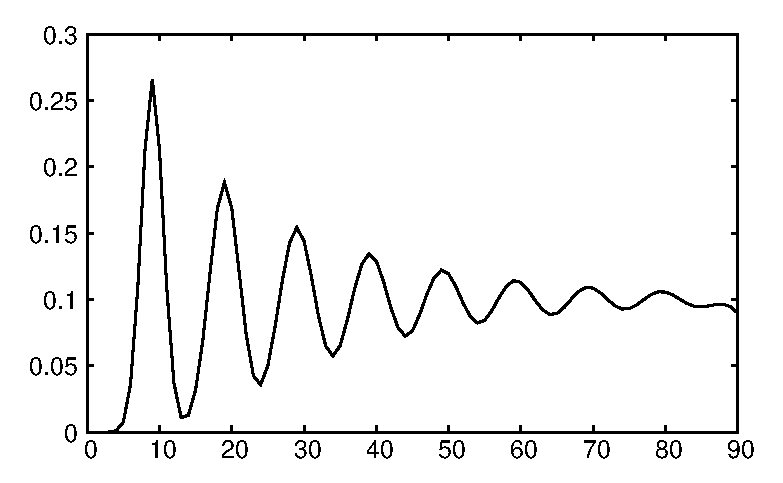
\includegraphics[width=0.7\textwidth]{images/example_pccf.eps}
	\caption{Pccf example}\label{fig:pccf_example}
\end{figure}


\section{Integration with Bayesian detector}


\section{Integration with CuSum}


%~\footnote{we useterms recurrent and reoccurring interchangebly}
% The difference to the previous work is that we calculate Pccf in a concise
% way using moment generating functions and we calculate it for several
% commonly used distributions used for inter arrival time modelling.
%In our previous work we applied threshold value to the calculated probability estimates, but now we found it much more practical just to use equally spaced time moments surrounded by time intervals of a fixed size.
% Probability estimates given by Pccf should be used to assess confidence intervals for predictions and for assessment of how many changes in the future we want to make a prediction for.

% Mgfs for commonly used for inter-arrival times modelling distributions are~\cite{wasserman2013all}
% as follows.
% for Exponential distribution with rate $\lambda$ it is $\frac{\lambda}{\lambda - t}$;
% and for the Gamma distribution $\Gamma(\alpha, \lambda)$ is $\Big ( \frac{1}{1- \lambda t} \Big )^{\alpha}$.
% $\Big (\frac{\lambda}{\lambda - t} \Big)^{\alpha}$ %([ref](http://math.tntech.edu/ISR/Introduction_to_Probability/Distributions_of_Functions/thispage/newnode11.html))
%
% % POSISSON is not needed, as we model inter-arrival times, not number of occurences
%\item Poisson is $e^{\lambda (e^t-1)}$
%
% $\mathbb{E}(e^{tX}) = \sum_{k=0}^{\infty} e^{tk} e^{-\lambda} \lambda^k/k! = e^{\lambda (e^t-1)}$
% https://en.wikipedia.org/wiki/Gamma_distribution#Summation
% https://stats.stackexchange.com/questions/51605/the-sum-of-two-independent-gamma-random-variables
% proof: https://en.wikipedia.org/wiki/Characteristic_function_%28probability_theory%29#Example
%Proof for the Gamma can be found \href{https://en.wikipedia.org/wiki/Characteristic\_function\_\%28probability\_theory\%29#Example}{here}. Characteristic functions are $\phi_X(t)=(1-\lambda i t)^{-a}$ and $\phi_Y(t)=(1-\lambda i t)^{-b}$. Therefore $\phi_{X+Y}(t) = (1-\lambda i t)^{-(a+b)}$.
%
% Poisson & $\mathbb{E}(e^{tX}) = \sum_{k=0}^{\infty} e^{tk} e^{-\lambda} \lambda^k/k! = e^{\lambda (e^t-1)}$ & Inter-arr. times are from Exp. And Pdf is for Gamma \\
%Weibull? & & p pp\\
% Gamma~\cite{wasserman2013all}
%
%  Corresponding Mgfs for the sums are as follows.
%  for Gamma distribution $M_{X+Y} (t) =  \Big (\frac{\lambda}{\lambda - t} \Big)^{a + b}$
%  and for Exponential distribution is $\frac{\lambda}{\lambda-t}$.
%
%  Gaussian,
%  If $X \sim N(\mu_X, \sigma_X)$ and $Y \sim N(\mu_Y,\sigma_Y)$ then $X+Y \sim N(\mu_X + \mu_Y, \sqrt{\sigma_X + \sigma_Y})$
%  $$M_{X+Y}(t) = \exp \Big ( t \mu_X  + \frac{\sigma_X^2 t^2}{2} \Big) \cdot \exp \Big ( t \mu_Y  + \frac{\sigma_Y^2 t^2}{2} \Big) = \exp \Big [ (\mu_X + \mu_Y) t + \frac{(\sigma_X^2 + \sigma_Y^2) t^2}{2} \Big ] $$ which is a characteristic function of the normal distribution with parameters $\mu =  \mu_X + \mu_Y$ and $ \sigma^2 = \sigma_X^2 + \sigma_Y^2$.
%
%
% $\Gamma(k, \lambda)$.
% Copied to for)thesis.tex
%
%\begin{itemize}
%	% POSISSON is not needed, as we model inter-arrival times, not number of occurences
%	%    %\item \textbf{For the Poisson.}
%	%$$M^P_{X+Y} (t) =  e^{\lambda (e^t-1)}  e^{\mu (e^t-1)} =  e^{(\lambda+\mu) (e^t-1)}$$
%	%It means $X+Y \sim \text{Poiss}(\lambda + \mu)$ (note: the sum of two Poissons is also a Poisson, which is not general for any distribution)
%	\item \textbf{Gaussian}
%	If $X \sim N(\mu_X, \sigma_X)$ and $Y \sim N(\mu_Y,\sigma_Y)$ then $X+Y \sim N(\mu_X + \mu_Y, \sqrt{\sigma_X + \sigma_Y})$
%	$$M_{X+Y}(t) = \exp \Big ( t \mu_X  + \frac{\sigma_X^2 t^2}{2} \Big) \cdot \exp \Big ( t \mu_Y  + \frac{\sigma_Y^2 t^2}{2} \Big) = \exp \Big [ (\mu_X + \mu_Y) t + \frac{(\sigma_X^2 + \sigma_Y^2) t^2}{2} \Big ] $$
%
%	which is a characteristic function of the normal distribution with parameters $(\mu =  \mu_X + \mu_Y, \sigma^2 = \sigma_X^2 + \sigma_Y^2)$.
%
%	\item \textbf{Gamma}
%	If $X \sim \Gamma(a, \lambda), Y \sim \Gamma(b, \lambda)$ then $X+Y \sim \Gamma(a+b, \lambda)$.
%
%	$$M_{X+Y} (t) = M_X (t) \cdot M_Y (t) = \Big (\frac{\lambda}{\lambda - t} \Big)^{a}  \Big (\frac{\lambda}{\lambda - t} \Big)^{b} =  \Big (\frac{\lambda}{\lambda - t} \Big)^{a + b}$$
%
%	\item \textbf{Exponential}
%	Mgf for the exponential distribution with $\lambda=1$ is $\frac{1}{1-t}$ where $t<1$.
%	% Lec.14 (Statistics 101): https://www.youtube.com/watch?v=Qjeswpm0cWY&index=24&list=PL2SOU6wwxB0uwwH80KTQ6ht66KWxbzTIo
%	% START: 23:27
%	% Using the property of moment generating functions (by definition)
%	% \[\psi_{X+Y}(t) = \mathbb{E}(e^{t (X+Y)}) = \mathbb{E}(e^{t X}) \mathbb{E} (e^{t Y})\]
%	Mgf for the $n$-th event $T_n = \sum_{j=1}^{n} X_j, \text{ where } X_j \sim e^{-\lambda t}$ is $\Big ( \frac{1}{1-t} \Big )^n$.
%	But Mgf for $Y \sim \Gamma(n,1)$ is also $\Big(\frac{1}{1-t} \Big)^n$.
%	Therefore if inter-arrival times are i.i.d. from the exponential distribution with parameter $\lambda$ the PDF for the k-th event is $\Gamma(k, \lambda)$.
%	%\begin{equation}
%	%    \mathbb{E}(e^{tY}) = \frac{1}{\Gamma(n)} \int_{0}^{\infty} e^{ty} y^{n} e^{-y} \frac{d y}{y} = \frac{1}{\Gamma(n)} \int_{0}^{\infty} y^n e^{-(1-t)y} \frac{d y}{y}
%	%\end{equation}
%	%Let, $x=(1-t)y$, then $d x = (1-t) d y$, then we get
%	%\begin{equation}
%	%    \mathbb{E}(e^{tY}) = \frac{(1-t)^{-n}}{\Gamma(n)} \int_{0}^{\infty} x^n e^{-x} \frac{d x}{x} = \Big(\frac{1}{1-t} \Big)^n
%	%    \label{eq:mgf_gamma_1}
%	%\end{equation}
%	%This is (Equation~\ref{eq:mgf_gamma_1}) the same Mgf as Mgf for the sum of i.i.d. from Exponential distribution with $\lambda=1$ (Equation~\ref{eq:mgf_exp_n}).
%
%	%If $X \sim Exp(\lambda_1)$ and $Y \sim Exp(\lambda_2)$ then $X+Y \sim $
%	%$$M^E_{X+Y}(t) = \frac{\lambda_1}{\lambda_1 - t} \frac{\lambda_2}{\lambda_2 - t}$$
%\end{itemize}


%, i.e.  $\sum_{k=1}^{N} P(t_k^{\text{CHP}} = t_i)$.
%	\begin{equation}
%		\text{Any } t_{k}^{\text{CHP}} = t_i
%		% \text{ or } t_{2}^{\text{CHP}} = t   \dots t_{k}^{\text{CHP}} = t
%		%C_1 = t \text{ or } C_2 = t \text{ or } \dots C_n = t
%		\label{eq:events_union}
%	\end{equation}
%Since events $t_k^{\text{CHP}} = t_i$ are disjoint Pccf can be calculated as
%\begin{equation}
%	\sum_{i=1}^{N} \sum_{k=1}^{N} P(t_k^{\text{CHP}} = t_i).
%\end{equation}
%\begin{equation}
%	P\Big(\bigcup\limits_{k=1}^{N} (t_k^{\text{CHP}} = t_i) \Big ) = \sum_{k=1}^{N} P(t_k^{\text{CHP}} = t_i)
%\end{equation} % Wasserman, page5



\section{Research questions}
% Nikolai: - Questions about ROI and PCCF
% Nikolai: - Questions about integration with detectors
% Nikolai: - Questions about impact of better detection of recurrent changes on model adaptation / adaptive learning
% Nikolai: - From the SDM, BLPA and the submitted journal paper please extract /formulate the main research questions they answer and add them here to Section 3.2
Change point detection in time series data and change point detection as drift detection method (DDM) as a control unit in adaptive ML system~\ref{fig:fig3_gama_survey_cd}.
Concept drifts are usually assumed to be not predictable.
We consider the case when they are predictable.
When predicting occurrence of a change point or CD event a number of assumptions is made.
Namely
\begin{itemize}
  \item The main assumption is an assumption about probability distribution of inter-arrival times between changes or CD events, and particular choice of parameters values of the distribution. 
  \item Assumptions about width of the region of interest (ROI) and its positioning relatevely to the changepoint (left, center, right).
  \item Assumption about number of events to be predicted, as with larger number the larger the uncertainty is due to mathematical properties of predictive confidence change function (Pccf).
\end{itemize}
What will happen if assumptions are wrong? And what are the benefits if correct?
Recurrency for change detection and recurrency for model adaptation.

Assumptions about statistical properties of the input signal for change detector. 

In this work we concentrate on the Change detection control unit (Figure~\ref{fig:fig3_gama_survey_cd}) which makes a decision when to retrain the model.
Implementation is done in a form of change detection algorithms.
In~\cite{XXX} we demonstrated how FA rate and detection delays can be lowered for changedetection problem if assumptions are correct.
It can be used for concept drift handling in on-line learning under certain assumptions.

\begin{itemize}

  \item Usually changes, or, concept drifts, are assumed to be not predictable. In this thesis we address to the question - can we increase change detection and prediction performance using information about temporal re-occurence patterns of changes? 

  \item How to formalize recurrency? As any sequence of events can be considered as recurrent. Answer - Assumptions about distributions of inter-arrival times.

  \item How to integrate Pccf with change detectors? What are the advantages / drawbacks of  Post- or pre-processing settings? Answer: detection delay reductions is possible only in pre-processing settings; Post-processing is more safe and only removes FAs.

  \item How to deal with uncertainty in assumptions? Answer - BLPA

  \item Assuming i) Model ii) Model with DDM iii) Model with DDM and embedded Pccf. Is it so that iii) is better than ii) and ii) is better than i) under certain assumptions (Figure~\ref{fig:research_question})? If assumptions are wrong then even ii) is not better than i)~\cite{SouzaRMB20}.

  \item What happens if Pccf predictions are not correct due to the data properties or due to the wrong assumptions/model? 

  \item How it can be used for model adaptation?

\end{itemize}

\begin{figure}[htb!]
	\centering
	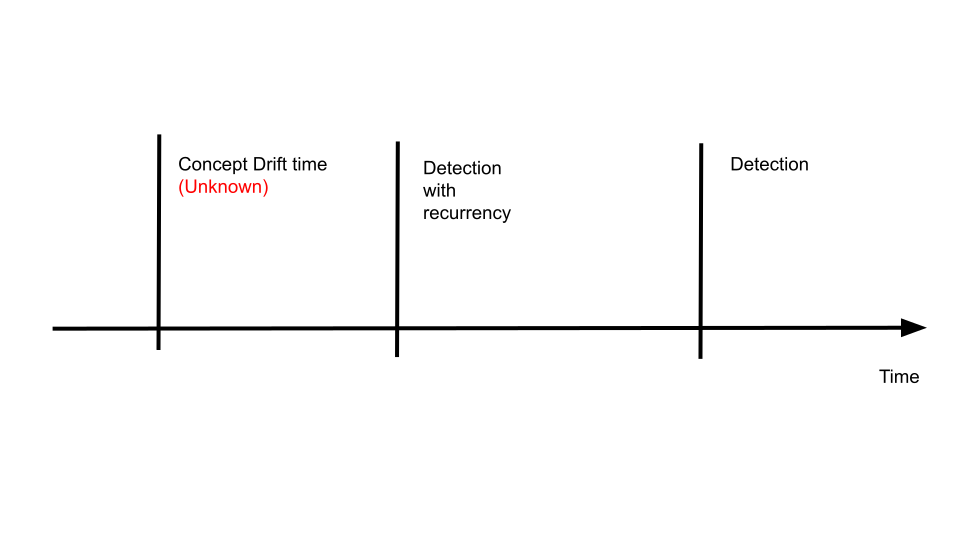
\includegraphics[width=0.9\textwidth]{images/google_slides/scheme_cd_recurrency}
  \caption{
	}\label{fig:research_question}
\end{figure}


\section{Research methodology}
%Nikolai:  Here, I think you can use a high-level umbrella or Nunamaker et al. 
%Nikolai:  See e.g. Figure 14 and brief discussion around it in my thesis at p.49  
% https://jyx.jyu.fi/bitstream/handle/123456789/13253/1/9513922715.pdf
%Nikolai:  You can adapt the figure to your needs. I.e. four ovals become:
%Nikolai:  Theory building: PCCF; (conceptualization, formalization, theorem proving
%Nikolai:  Artifact development: Recurrent change detection technique development
%Nikolai:  Experimentation with benchmark datasets: (recurrent) change detection performance; effect of (recurrent) change detection on predictive modeling
%Nikolai:  
%Nikolai:  Simulation with synthetic data: (recurrent) change detection performance
%Nikolai:  Please put as much info into Chapter 3 as you can during tomorrow. F


% section Datasets
\section{Datasets}

In papers~\cite{MaslovSDM2016, MaslovIJCNN2017} we performed experiments experiments with artificially generated and with real datasets.

In the paper~\cite{MaslovSDM2016} we did experiments with two real datasets - with i) the boiler dataset containing sensor readings measuring recurrent refuelling behavior and ii) Internet traffic dataset\footnote{\url{https://datamarket.com/data/list/?q=internet+traffic+data+price\%3Afree}} containing aggregated internet traffic data from Internet Service Provider in the UK academic network backbone. The data series is illustrate in Figure~\ref{fig:trafficdata}.

In the paper~\cite{MaslovIJCNN2017} we used the Human activity data set~\cite{reyes2016transition} which contains sensor measurements from people performed 6 types of activities: three static postures (standing, sitting, lying) and three dynamic activities (walking, walking downstairs and walking
upstairs).

In the Journal version paper (cite) we did experiments with the time series of temperature measurements collected from the sensor installed in the home office environment.




\begin{itemize}
  \item 
  \item CFB in~\cite{x}
  \item Temperature signal from sensor
\end{itemize}

